\chapter{Decision Trees}
\label{ch:decision-trees}

\chapterguide%
  {\chapref{ch:training} plus basic probability from \chapref{ch:statistics}; entropy is helpful but re-explained here.}
  {compute Gini impurity and information gain by hand; choose a split on real counts; read a fitted tree as rules; control depth and pruning; and treat feature importance with care.}

In the game of Twenty Questions you never ask ``is it a giraffe?'' first. You ask a question that splits the possibilities well, such as ``is it alive?'', and then ask the next one depending on the answer. A decision tree plays that game with a table. It routes each row through questions such as ``age below 30?'' until it reaches a \term{leaf}, which holds the prediction. Small trees can be read aloud, and forests and boosting combine many of them into stronger models (\chapref{ch:ensembles}).

\begin{utpfig}[A small decision tree]{A small decision tree. Each internal node asks one question about one feature, and each leaf makes a prediction.}{fig:tree-example}
\begin{tikzpicture}[
  font=\small,
  qnode/.style={draw, rounded corners=2pt, align=center, fill=UTPPaleBlue, inner sep=4pt},
  leaf/.style={draw, align=center, inner sep=4pt},
  level distance=1.35cm,
  level 1/.style={sibling distance=4.6cm},
  level 2/.style={sibling distance=2.4cm},
  edge from parent/.style={draw, -{Stealth[length=1.8mm]}}
]
\node[qnode] {age $<30$?}
  child {node[qnode] {income $\geq 50$k?}
    child {node[leaf] {predict:\\approve}
      edge from parent node[left=1pt] {yes}}
    child {node[leaf] {predict:\\review}
      edge from parent node[right=1pt] {no}}
    edge from parent node[left=2pt] {yes}}
  child {node[leaf] {predict:\\approve}
    edge from parent node[right=2pt] {no}};
\end{tikzpicture}
\end{utpfig}

\section{How a tree is grown}
\label{sec:decision-tree}

Standard tree learning (the CART algorithm) is \term{greedy and recursive}:

\begin{enumerate}
  \item At the current node, consider candidate splits: for a numerical feature, thresholds between sorted values; for categorical features, the rules depend on the implementation; scikit-learn expects them one-hot encoded, which is what Lab~3 does.
  \item Score each candidate by how much it \emph{purifies} the data --- how well it separates the classes (or, for regression, how much it shrinks the spread of the label).
  \item Apply the best split, sending observations left and right.
  \item Repeat on each child until a stopping rule fires; each final node becomes a leaf that predicts its majority class (classification) or mean label (regression).
\end{enumerate}

Greedy means the algorithm never looks ahead or reconsiders: it takes the best immediate split at every step. That keeps training fast and usually works well, though it does not guarantee the globally best tree.

\section{Measuring impurity}

\begin{analogy}
Picture a bag of red and blue marbles. A bag of one color is pure, so you can name the color of the next marble with no doubt. A half-and-half bag is as mixed as it gets. A good question pours one mixed bag into two bags, each purer than the original.
\end{analogy}

To pick a split, the algorithm needs a number for ``how mixed is this node?'' With $p_k$ the fraction of class $k$ in a node, two standard measures are the \term{Gini impurity} and the \term{entropy}:
\[
  G=1-\sum_{k=1}^{K}p_k^2,
  \qquad
  H=-\sum_{k=1}^{K}p_k\log_2 p_k.
\]
Both are zero for a pure node (one class only) and largest for a perfect mixture. Gini reads as ``the probability of mislabeling a random point if labels were assigned according to the node's class mix''; entropy reads as ``how many yes/no questions of uncertainty remain.'' A split is chosen to maximize the \term{information gain}: the parent's impurity minus the size-weighted impurity of the children,
\[
  \operatorname{Gain}
  =I(\text{parent})
  -\frac{n_{\mathrm{left}}}{n}I(\text{left})
  -\frac{n_{\mathrm{right}}}{n}I(\text{right}),
\]
where $I$ is either measure. Gini and entropy almost always agree on the best split; Gini is slightly cheaper to compute and is the common default.

\begin{workedexample}
A node holds 10 loan applications: 6 approved ($+$) and 4 rejected ($-$). Its Gini impurity is
$G_{\text{parent}}=1-(0.6^2+0.4^2)=0.48$.

\emph{Candidate split A} produces children $[4+,0-]$ and $[2+,4-]$:
\[
  G_{\text{left}}=0,
  \qquad
  G_{\text{right}}=1-\left[{\left(\tfrac{1}{3}\right)}^2+{\left(\tfrac{2}{3}\right)}^2\right]=\tfrac{4}{9}\approx 0.444,
\]
\[
  \operatorname{Gain}_A
  =0.48-\left(\tfrac{4}{10}\times 0+\tfrac{6}{10}\times 0.444\right)
  =0.48-0.267=0.213.
\]

\emph{Candidate split B} produces children $[3+,2-]$ and $[3+,2-]$. Each child has the same $60/40$ mix as the parent, so each has $G=0.48$, the weighted impurity is unchanged, and $\operatorname{Gain}_B=0$: split B tells us nothing, and split A wins. (Entropy agrees: split A's gain is $0.971-0.551\approx 0.42$ bits.)
\end{workedexample}

\section{Finding the best split, on real data}

Evaluate every candidate question, and keep the one with the largest weighted drop in impurity. If a threshold separated two classes perfectly, both children would be pure and the gain would equal the parent's impurity.

\keepspace{16\baselineskip}
\begin{workedexample}
The Titanic table has 549 deaths and 342 survivors, so its Gini is $1-(0.616^2+0.384^2)=0.473$. Four candidate first questions:

\medskip
\centering\small
\begin{tabular}{@{}lccccc@{}}
\toprule
\rowcolor{UTPPaleBlue!92}
\utpth{Question} & \utpth{Yes: died, lived} & \utpth{Gini} & \utpth{No: died, lived} & \utpth{Gini} & \utpth{Gain} \\
\midrule
Sex is female? & 81, 233 & 0.383 & 468, 109 & 0.306 & \textbf{0.140} \\
Class is third? & 372, 119 & 0.367 & 177, 223 & 0.493 & 0.049 \\
Fare at most 15? & 344, 114 & 0.374 & 205, 228 & 0.499 & 0.039 \\
Embarked at C? & 75, 93 & 0.494 & 474, 249 & 0.452 & 0.013 \\
\bottomrule
\end{tabular}
\par\raggedright
\medskip
Check the first row: 314 women and 577 men, so the weighted child impurity is $\frac{314}{891}(0.383)+\frac{577}{891}(0.306)=0.333$, and the gain is $0.473-0.333=0.140$. Sex wins by a wide margin, and it is the question Lab~3's tree asks first. Then the same search repeats inside each child. Lab~3's tree goes on to ask about age among men and about class among women.
\end{workedexample}

\begin{libnote}
Observed-value and midpoint thresholds can partition training rows identically despite different printed values.
\end{libnote}

\section{The geometry: rectangles in feature space}

Because every question compares one feature to one threshold, a tree carves feature space into axis-aligned rectangles, one per leaf, and predicts a constant inside each.

\begin{utpfig}[A tree carves feature space into rectangles]{A tree carves feature space into axis-aligned rectangles. The first split is $x_1<3$, the second splits only the left side at $x_2<2$, and each region predicts a constant.}{fig:tree-rectangles}
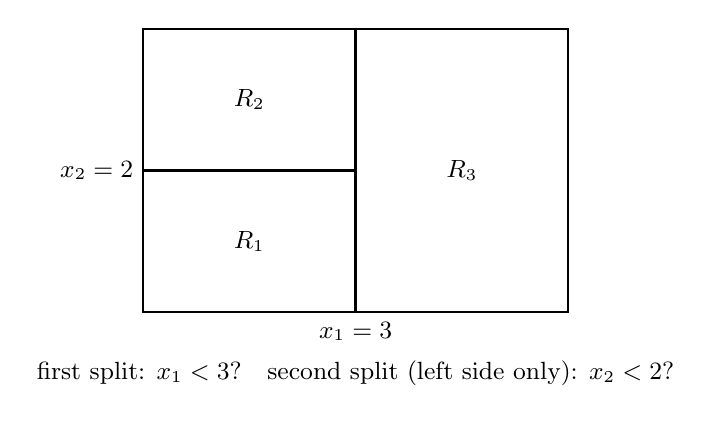
\begin{tikzpicture}[scale=0.9, font=\small]
\draw[thick] (0,0) rectangle (6,4);
\draw[thick] (3,0) -- (3,4);
\draw[thick] (0,2) -- (3,2);
\node at (1.5,1) {$R_1$};
\node at (1.5,3) {$R_2$};
\node at (4.5,2) {$R_3$};
\node[below] at (3,0) {$x_1=3$};
\node[left] at (0,2) {$x_2=2$};
\node[below] at (3,-0.55) {first split: $x_1<3$?\quad second split (left side only): $x_2<2$?};
\end{tikzpicture}
\end{utpfig}

Axis-aligned rules fit naturally; diagonal boundaries require staircases of splits.

\section{Regression trees}

Regression trees choose splits that reduce within-node variance. Each leaf predicts its training-label mean, producing a piecewise-constant function.

\begin{workedexample}
Labels $\{2,3,10,11\}$ have mean $6.5$ and variance $16.25$. Splitting into $\{2,3\}$ and $\{10,11\}$ reduces weighted variance to $0.25$; leaves predict $2.5$ and $10.5$.
\end{workedexample}

\begin{workedexample}
The best single question for the study log is ``hours at most 17?''. Its leaves predict 60.0 for the eight students below and 40.5 for the two above. Ask this tree about someone who studied 100 hours, and it still says 40.5.
\end{workedexample}

Leaf means stay within the range of the training labels, so ordinary regression trees do not extrapolate. Lab~2 runs into this: its bike-demand forest under-predicts a busy autumn.

\section{Stopping and pruning}

Unrestricted growth can produce pure leaves and memorize observations. Use two complementary controls:

\begin{utptable}
\renewcommand{\arraystretch}{1.16}
\setlength{\tabcolsep}{5pt}
\begin{tabularx}{\linewidth}{@{}>{\footnotesize\bfseries\leavevmode\color{UTPNavy}}m{0.22\linewidth}>{\footnotesize}m{0.40\linewidth}>{\footnotesize}X@{}}
\toprule
\rowcolor{UTPPaleBlue!92}
\utpth{Method} & \utpth{How it works} & \utpth{Trade-off} \\
\midrule
Pre-pruning (early stopping) & Refuse to grow past limits set in advance: a maximum depth, a minimum number of observations required to split a node or to sit in a leaf, or a minimum impurity decrease. & Simple and fast; the limits are hyperparameters tuned on validation data. \\
Post-pruning & Grow a deliberately large tree first, then cut back branches whose contribution does not justify their complexity. \term{Cost-complexity pruning} charges a penalty $\alpha$ per leaf and keeps the subtree that best trades training fit against size; $\alpha$ is chosen by cross-validation. & Growing and then cutting can rescue good splits that become visible only after a mediocre one, which early stopping would never discover. \\
\bottomrule
\end{tabularx}
\end{utptable}

\section{Depth: the dial between too simple and memorized}

Tree depth controls the bias--variance trade-off from \secref{sec:bias-variance}. Lab~3 measures it on the Titanic (\figref{fig:tree-depth}).

\begin{utpfig}[Depth and the bias--variance trade-off]{Accuracy of Titanic trees by depth, on the rows they trained on and on 223 validation rows. Training accuracy climbs with every level, while validation accuracy peaks at depth 3 (0.785) and then drifts down to 0.731.}{fig:tree-depth}
\begin{tikzpicture}
\begin{axis}[logaxis, width=0.72\linewidth, height=5.0cm, xlabel={max\_depth}, ylabel={accuracy}, xmin=0.5, xmax=12.5, ymin=0.7, ymax=1.0,
  xtick={1,2,...,12}, ytick={0.7,0.8,0.9,1.0}, legend style={at={(0.03,0.97)},anchor=north west}]
\addplot[draw=UTPBlue,mark=*,mark size=1.3pt,thick] coordinates {(1,0.793)(2,0.808)(3,0.832)(4,0.852)(5,0.868)(6,0.882)(7,0.892)(8,0.913)(9,0.927)(10,0.939)(11,0.948)(12,0.954)};
\addlegendentry{training}
\addplot[draw=UTPOrange,mark=square*,mark size=1.3pt,thick] coordinates {(1,0.767)(2,0.758)(3,0.785)(4,0.776)(5,0.767)(6,0.771)(7,0.767)(8,0.74)(9,0.749)(10,0.74)(11,0.74)(12,0.731)};
\addlegendentry{validation}
\end{axis}
\end{tikzpicture}
\end{utpfig}

Left to grow without limit, the same tree reaches depth 21 with 146 leaves. It scores 0.978 on its training rows and 0.722 on validation: it has started describing individual passengers instead of patterns.

\subsection{The controls that limit growth}

\begin{utptable}
\begin{tabularx}{\linewidth}{@{}>{\bfseries\leavevmode\color{UTPNavy}\ttfamily}m{0.25\linewidth}X@{}}
\toprule
\rowcolor{UTPPaleBlue!92}
\utpth{Setting} & \utpth{What it does} \\
\midrule
max\_depth & Hard limit on how many questions can be asked in a row. \\
min\_samples\_split & Refuse to split a node holding fewer than this many rows. \\
min\_samples\_leaf & Every final leaf must contain at least this many rows. \\
max\_leaf\_nodes & Cap the total number of leaves. \\
ccp\_alpha & Cost-complexity pruning: grow fully, then prune back. \\
class\_weight & Make rare-class rows count for more. \\
\bottomrule
\end{tabularx}
\end{utptable}

\subsection{Cost-complexity pruning, properly}

Grow the tree until every leaf is pure or tiny. Then define, for a penalty $\alpha\ge0$, the score
\[
  \text{(training impurity of the subtree)}+\alpha\times\text{(number of leaves)}.
\]
Increasing $\alpha$ trades fit for fewer leaves along a nested pruning path. Cross-validate \texttt{ccp\_alpha}; unlike a uniform depth limit, pruning retains detail where useful.

\section{Strengths, limitations, and practical notes}

\begin{itemize}
  \item \term{Interpretability:} the model \emph{is} an explanation; individual predictions can be justified by reading off the path.
  \item \term{Preprocessing:} numerical trees need no scaling; categorical and missing-value handling depends on the implementation.
  \item \term{Nonlinearity for free:} interactions and thresholds emerge automatically, with no feature engineering.
  \item \term{Instability:} small data changes can alter early splits and whole subtrees, motivating the ensembles in \chapref{ch:ensembles}.
  \item \term{Feature importance:} use the interpretation and bias cautions in \secref{sec:tree-feature-importance}.
\end{itemize}

\begin{keyidea}
Trees learn readable nonlinear rules through impurity reduction. Their instability also makes them useful base learners for ensembles.
\end{keyidea}

\recipecard{Decision tree}{A sequence of yes/no questions, each about one feature, ending in leaves that predict a constant.}{Gini impurity or entropy for classes; squared error for numbers.}{Greedy search: at each node, take the best split available now, and never look back.}

\begin{modelcard}{Decision Trees - Quick Guide}
\begin{tabularx}{\linewidth}{@{}>{\bfseries\leavevmode\color{UTPNavy}}p{0.24\linewidth}X@{}}
Best when & Nonlinear rules, interactions, mixed feature scales, and human-readable if-then paths are useful. \cr
Preprocessing & Usually no scaling is needed; categories still need a supported representation; missing-value handling depends on the implementation. \cr
Main controls & Maximum depth, minimum samples per split/leaf, maximum leaf nodes, and pruning strength. \cr
Strengths & Handles nonlinear relationships and interactions; predictions are easy to trace through a small tree. \cr
Watch for & High variance, unstable splits, misleading feature importance, and blocky extrapolation. \cr
\end{tabularx}
\end{modelcard}

\section{Interpreting a fitted tree}

Inspect paths and leaf counts. Lab~3's Titanic tree splits first on \texttt{Sex}, then \texttt{Age} for men and \texttt{Pclass} for women.

\begin{keyidea}
The printed paths are the model's actual rules, not a post-hoc approximation. Readability alone does not establish fairness, causality, stability, or safety.
\end{keyidea}

\section{Feature importance, and why to distrust it}
\label{sec:tree-feature-importance}

\term{Impurity importance} sums a feature's impurity reductions. Two cautions:

\begin{itemize}
  \item Many candidate thresholds can inflate importance, favoring continuous features over binary ones.
  \item Correlated features can substitute for one another, making importance unstable.
\end{itemize}

\term{Permutation importance} is the safer alternative: shuffle one feature's values in the validation data and measure how much the score drops. A large drop means this fitted model relied on that column. It is computed on held-out rows, so it also reflects generalization rather than training fit.

\begin{keyidea}
Feature importance describes which columns this fitted model used. Apply the general association-versus-causation rule from \secref{sec:correlation}; importance is not causal evidence.
\end{keyidea}

\begin{debugtask}
A depth-20 tree has nearly perfect training accuracy and unstable feature importance across random splits. Diagnose the likely failure mode, then compare depth 2, 5, and 20 using identical validation folds and a sealed test set.
\end{debugtask}

\begin{decisionmemo}
Choose between a shallow single tree and a random forest for a decision that must be explained to a nontechnical reviewer. Your memo must separate predictive performance from interpretability and state what level of performance loss, if any, you would accept for the simpler model.
\end{decisionmemo}

\begin{chapterrecap}
\begin{itemize}
  \item A tree asks one question at a time and predicts a constant in each leaf, carving the space into rectangles.
  \item Each split is chosen greedily, to reduce impurity the most. Gini and entropy almost always agree.
  \item On the Titanic the first question is sex, with a gain of 0.140, far ahead of class or fare.
  \item Unlimited depth memorizes: training accuracy reached 0.978 with validation at 0.722. Limit growth or prune, and tune on validation.
  \item Importance scores describe this fitted model. They are unstable under correlation, and they are not causes.
\end{itemize}
\end{chapterrecap}

\begin{quickcheck}
\begin{enumerate}
  \item What does a decision-tree split try to improve at each node?
  \item A node holds 8 positives and 2 negatives. What is its Gini impurity? A split gives children of $[4+,0-]$ and $[4+,2-]$; what is the gain?
  \item Why can an unconstrained tree achieve excellent training performance yet generalize poorly?
  \item Why are ordinary decision trees largely insensitive to monotonic rescaling of a numerical feature?
  \item Why can a regression tree not predict a mark above the highest mark it trained on?
\end{enumerate}
\end{quickcheck}

\begin{checkanswers}
\begin{enumerate}
  \item The purity of the children compared with the parent, as measured by the weighted drop in Gini or entropy (or in variance, for regression).
  \item Parent: $1-(0.8^2+0.2^2)=0.32$. The left child is pure. The right child: $1-[(2/3)^2+(1/3)^2]=0.444$. Weighted child impurity: $0.6\times0.444=0.267$. Gain: $0.32-0.267=0.053$.
  \item With enough depth it can give every row its own leaf. Those last splits describe individual rows, which is why training accuracy rises to 0.978 while validation falls to 0.722 on the Titanic.
  \item A split depends only on the order of the values, and stretching a column keeps its order, so the same rows go left and right.
  \item Each leaf predicts the mean of its training labels, and a mean cannot exceed the largest value in it.
\end{enumerate}
\end{checkanswers}
